\documentclass{sig-alternate}
%\documentclass[a4paper,10pt]{article}
\usepackage[utf8]{inputenc}
%El template pincha con spanish babel
%\usepackage[spanish]{babel}
\usepackage{amsmath, amssymb, amsfonts}
\usepackage{soul}
\usepackage{graphicx}
\usepackage{fancybox}
\usepackage[table]{xcolor}
\usepackage{soul}

\newtheorem{theorem}{Teorema}

\title{Banzai Totsugeki} 

\numberofauthors{4}
\author{
\alignauthor
Pose, Alberto Miguel\\
       \affaddr{Instituto Tecnol\'ogico de Buenos Aires}\\
       \affaddr{Buenos Aires, Argentina}\\
       \email{apose@alu.itba.edu.ar}
\alignauthor
Catalano, Juan Ignacio\\
       \affaddr{Instituto Tecnol\'ogico de Buenos Aires}\\
       \affaddr{Buenos Aires, Argentina}\\
       \email{jcatalan@alu.itba.edu.ar}
\and
\alignauthor 
Palombo, Mart\'in\\
       \affaddr{Instituto Tecnol\'ogico de Buenos Aires}\\
       \affaddr{Buenos Aires, Argentina}\\
       \email{mpalombo@alu.itba.edu.ar}
\alignauthor 
V\'azquez, Santiago Jos\'e\\
       \affaddr{Instituto Tecnol\'ogico de Buenos Aires}\\
       \affaddr{Buenos Aires, Argentina}\\
       \email{savazque@alu.itba.edu.ar}
}

\date{}

\begin{document}

\maketitle

\begin{abstract}
ABASTRAEEME
\end{abstract} 

\newpage

\section{Introducci\'on}

PONER QUE TIENE QUE CUMPLIR CADA METODO indep uniform
\section{Atacando a L'Ecuyer}
\label{sec:goingdown}

Se realiza un an\'alisis del generador de L'Ecuyer mediante los tests
Chi cuadrado(para analizar uniformidad) y Kolmogorov-Smirnov
(para analizar independecia).
Se hace una realizaci\'on de $10000$ muestras del generador de L'Ecuyer y se realian dichos tests.
Cabe destacar que para la realizaci\'on del generador de L'Ecuyer se utilizan las semillas 1 y 1 y
se agrupa dicha realizaci\'on en $10$ intervalos de clase. Los resultados de dicha realizaci\'on 
se observan en la figura \ref{fig:histograma_ecuyer}

\begin{figure}[ht]
\label{fig:histograma_ecuyer}
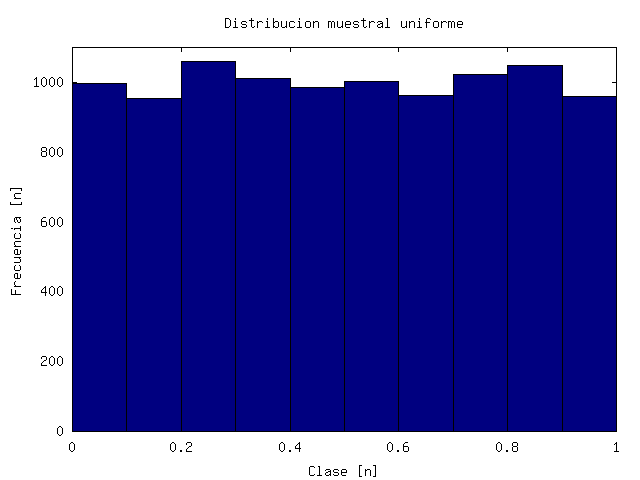
\includegraphics[width=8cm]{histograma_ecuyer}
\caption{Histograma de los 1000 n\'umeros agrupados en 10 intervalos de clase}
\end{figure}

\subsection{Test Chi Cuadrado}
\label{sec:chi}
Se aplica el test de Chi Cuadrado y se obtiene el estad\'istico $\chi_{0}^{2}=0.010003$.
Entonces, para $9$ grados de libertad y una significaci\'on de $\alpha=0.05$ se obtiene
el valor cr\'itico $\chi_{9,0.05}^{2}=16.92$.
Como $\chi_{0}^{2}=0.010003 < \chi_{9,0.05}^{2}=16.92$ se acepta la hip\'otesis $H_{0}$
de que la muestra provenga de una distribuci\'on uniforme.

\subsection{Test Kolmogorov-Smirnov}
\label{sec:kolmogorov}
Se aplica el test de Kolmogorov-Smirnov y se obtiene $D=0.99980$.
Para un nivel de significaci\'on $\alpha=0.05$ y $10$ intervalos de clase
se obtiene $D_{0.05}=0.410$. Entonces como $D > D_{\alpha}$
se acepta la hip\'otesis $H_{0}$ de que la muestra
provenga de una distribuci\'on uniforme.

\subsection{L'Ecuyer al desnudo}
Aunque el generador haya pasado los tests observados en las secciones \ref{sec:chi} y \ref{sec:kolmogorov}
es necesario ver como estan distribuidos los n\'umeros generados en el espacio. En todo GLC,
los n\'umeros generados yacen sobre hiperplanos (rectas en 2D, planos en 3D) bien definidos. Esto
sucede dado a la correlaci\'on entre los valores sucesivos del generador.
Sin embargo, si se posee un buen GLC, dichos hiperplanos son casi irreconocibles. Es por esto,
que se presenta la gr\'afica \ref{fig:ecuyer_2D} para observar lo que sucede en 2D.
Se puede observar que la gr\'afica se asemeja a una nube de puntos sobre la cual es
pr\'acticamente imposible distinguir recta alguna. \\


\begin{figure}[ht]
\label{fig:ecuyer_2D}
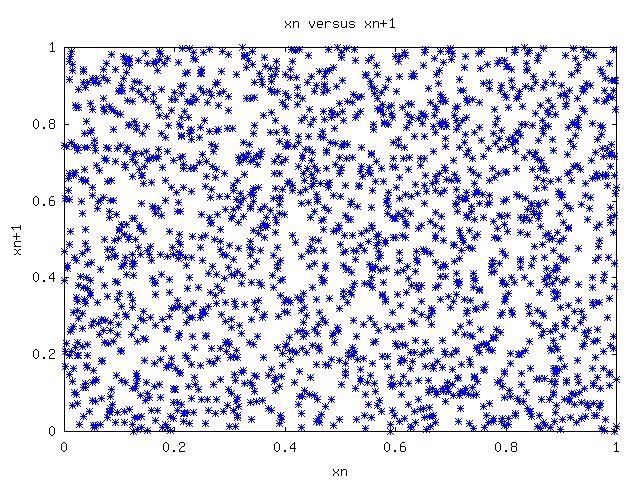
\includegraphics[width=8cm]{ecuyer2D}
\caption{Gr\'afica de $x_{n}$ versus $x_{n+1}$}
\end{figure}

Se repite el an\'alisis para 3D pero se toma el cuidado especial de genrar tres gr\'aficos rotados
para analizar lo que sucede en cada reg\'on. De este an\'alisis se obtienen las gr\'aficas
\ref{fig:ecuyer_3D_1}, \ref{fig:ecuyer_3D_2} y \ref{fig:ecuyer_3D_3}. Se puede observar
tambi\'en en este caso que no puede visualizarse ning\'un plano sobre la nube de puntos. \\

%TODO poner las perspectivas

\begin{figure}[ht]
\label{fig:ecuyer_3D_1}
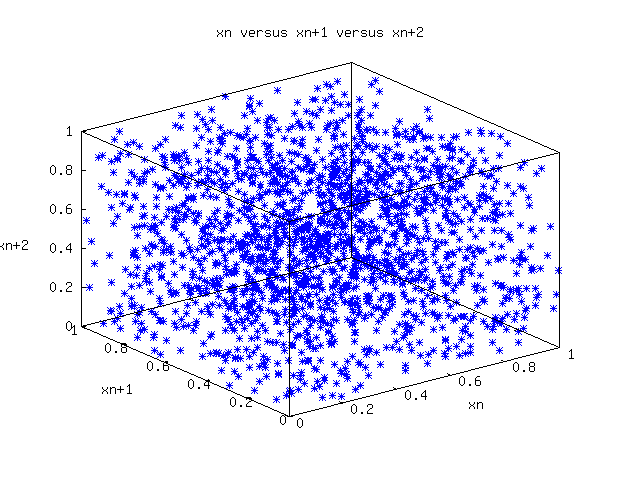
\includegraphics[width=8cm]{ecuyer3D_1}
\caption{Gr\'afica de $x_{n}$ versus $x_{n+1}$ versus $x_{n+2}$}
\end{figure}

\begin{figure}[ht]
\label{fig:ecuyer_3D_2}
%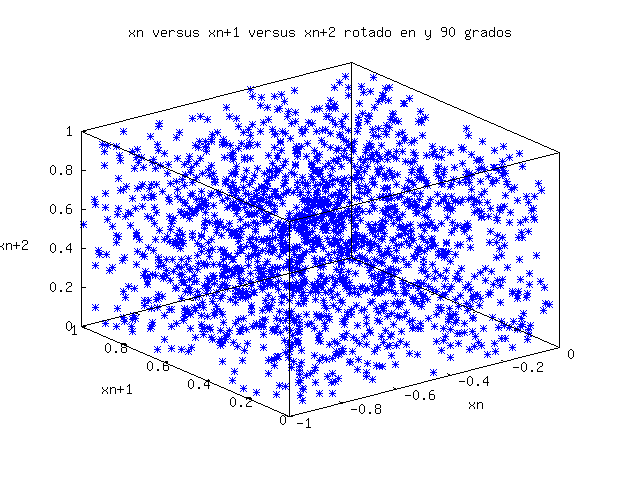
\includegraphics[width=8cm]{ecuyer3D_2}
\caption{Gr\'afica de $x_{n}$ versus $x_{n+1}$ versus $x_{n+2}$}
\end{figure}

\begin{figure}[ht]
\label{fig:ecuyer_3D_3}
%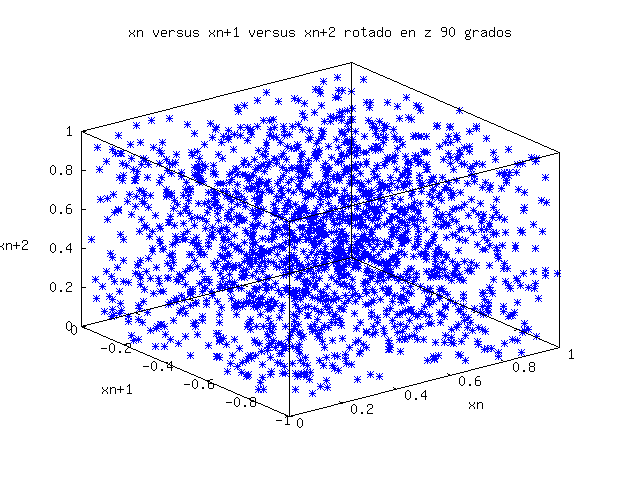
\includegraphics[width=8cm]{ecuyer3D_3}
\caption{Gr\'afica de $x_{n}$ versus $x_{n+1}$ versus $x_{n+2}$}
\end{figure}

Sin embargo, no se puede concluir que el generador de L'Ecuyer es un buen generador de n\'umeros
pseudoaleatorios. Sino, que ha pasado los tests Chi Cuadrado, Kolmogorov-Smirnov y que en sus
gr\'aficas no se presentan hiperplanos.

\section{Transformando a L'Ecuyer}
\label{sec:triangle}

A partir del generador de L'Ecuyer se desea obtener un generador de n\'umeros
pseudoaleatorios distribuidos seg\'un una funci\'on densidad triangular.\\
Para realizar \'esto se utiliza la t\'ecnica de la transformada inversa.

\begin{figure}[ht]
\begin{theorem}
\label{theo:1}
Sea $X$ una variable aleatoria con funci\'on de distribuci\'on $F(x)$
y se define:
$$U=F(X)$$
entonces $U$ es una variable aleatoria uniformemente distribuida en el intervalo $(0,1)$.
\end{theorem}
\end{figure}

Dicha t\'ecnica est\'a basada en el teorema \ref{theo:1} y consiste
en, dado un n\'umero $u$ que es una realizaci\'on de $U\sim\mathcal{U}[0,1]$,
entonces $x = F^{-1}(u)$ es una realizaci\'on de una VA $X$ con funci\'on
distribuci\'on $F(x)$.\\

La funci\'on de densidad triangular es \eqref{eq:triangle}. Su gr\'afica se observa
en la figura \ref{fig:triangle_fun}. A partir de ella podemos obtener
la funcio\'on distribuci\'on de probabilidad de $X$
\eqref{eq:triangleDistribution}.


\begin{figure}[ht]
\label{fig:triangle_fun}
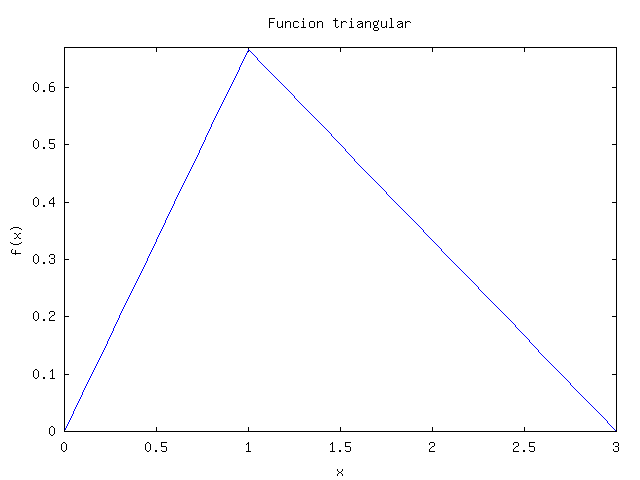
\includegraphics[width=8cm]{triangular}
\caption{Funci\'on de densidad triangular para $a=0$, $b=1$ y $c=3$}
\end{figure}


\begin{equation}
\label{eq:triangle}
f_{X}(x) =
\begin{cases}
\frac{2(x-a)}{(b-a)(c-a)} \quad & \text{si } a \leq x \leq b \\
\frac{2(c-x)}{(c-b)(c-a)} \quad & \text{si } b < x \leq c \\
0 \quad & \text{en otro caso}
\end{cases}
\end{equation}

\begin{equation}
\label{eq:triangleDistribution}
F_{X}(x) =
\begin{cases}
\frac{(x-a)^{2}}{(b-a)(c-a)} \quad & \text{si } a \leq x \leq b \\
\frac{b-a}{c-a} + \frac{(x-b)(2c-x+b)}{(c-a)(c-b)} \quad & \text{si } b < x \leq c \\
1 \quad & \text{en otro caso}
\end{cases}
\end{equation}

Dada dicha funci\'on hallamos su inversa \eqref{eq:inverse}.\\

\begin{equation}
\label{eq:inverse}
F^{-1}_{X}(u) =
\begin{cases}
\sqrt{u(b-a)(c-a)}+a \quad & \\
\text{si } 0 \leq u \leq \frac{b-a}{c-a} & \\
-\sqrt{-u(c-a)(c-b)+(b-a)(c-b)+(c-b)^{2}} + c \quad & \\
\text{si } \frac{b-a}{c-a} < u \leq \frac{c-b}{c-a}+\frac{b-a}{c-a} \\
\end{cases}
\end{equation}

Luego, el algoritmo consiste en generar un n\'umero pseudoaleatorio $u$ utilizando
un generador de n\'umeros pseudaleatorios con distribuci\'on uniforme en el $[0,1]$ (como el generador de L'Ecuyer).
Finalmente, con $u$ se obtiene $F^{-1}_{X}(u)$ que es una realizaci\'on de la variable aleatoria $X$.
Los resultados obtenidos se pueden observar en la figura \ref{fig:triangle}.

\begin{figure}[ht]
\label{fig:triangle}
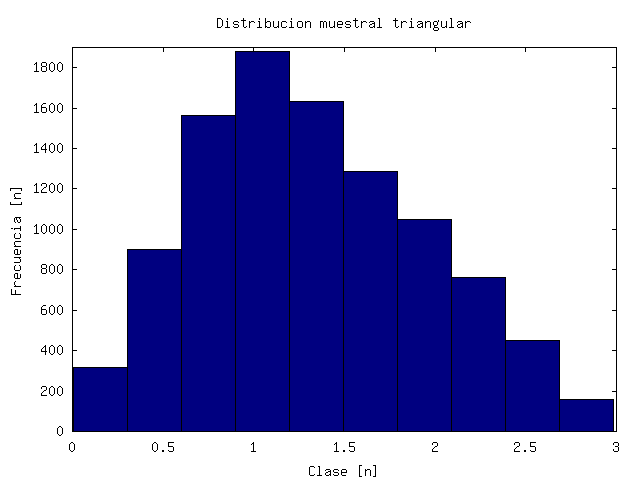
\includegraphics[width=8cm]{histograma_triangular}
\caption{Histograma de los n\'umeros obtenidos agrupados en 10 intervalos de clase}
\end{figure}

\newpage

\section{Resultados Conclusiones}
\label{sec:conclusiones}

%PONER QUE CHI SALE DE http://www.wiphala.net/research/manual/statistic/chi_cuadrado.html
%PONER QUE LOS DATOS DE KOLMOGOROV SE SACAN DE http://www.eridlc.com/onlinetextbook/appendix/table7.htm

\end{document}
